\documentclass[11pt]{scrartcl}

%%%%%%%%%%%%%%%%%%%%%%%%%%%%%%%%%
%% Ersetzen Sie in den folgenden Zeilen die entsprechenden -Texte-
%% mit den richtigen Werten.
\newcommand{\theNumber}{A203}
\newcommand{\theName}{Run-Length-Encoding}

\newcommand{\nameone}{Lukas Legner}
\newcommand{\nametwo}{Marlo Nickol}
\newcommand{\namethree}{Fabian Thomas-Barein}
%%%%%%%%%%%

\usepackage[utf8x]{inputenc}
\usepackage[ngerman]{babel}
\usepackage[T1]{fontenc}
\usepackage{amsmath}

\usepackage[babel,german=quotes]{csquotes}
\usepackage{graphicx}
\usepackage{color}
%\usepackage{here}
\usepackage{listings}
\usepackage{color}
\usepackage{microtype}
\usepackage{tikz}
\usetikzlibrary{shapes}

\setlength{\parindent}{0cm}

\definecolor{dkgreen}{rgb}{0,0.6,0}
\definecolor{gray}{rgb}{0.5,0.5,0.5}
\definecolor{mauve}{rgb}{0.58,0,0.82}
\lstset{ %
  language=Octave,                % the language of the code
  basicstyle=\footnotesize,           % the size of the fonts that are used for the code
  numbers=left,                   % where to put the line-numbers
  numberstyle=\tiny\color{gray},  % the style that is used for the line-numbers
  numbersep=5pt,                  % how far the line-numbers are from the code
  backgroundcolor=\color{white},      % choose the background color. You must add \usepackage{color}
  showspaces=false,               % show spaces adding particular underscores
  showstringspaces=false,         % underline spaces within strings
  showtabs=false,                 % show tabs within strings adding particular underscores
  frame=single,                   % adds a frame around the code
  rulecolor=\color{black},
  tabsize=2,                      % sets default tabsize to 2 spaces
  captionpos=b,                   % sets the caption-position to bottom
  breaklines=true,                % sets automatic line breaking
  breakatwhitespace=false,        % sets if automatic breaks should only happen at whitespace
  title=\lstname,                   % show the filename of files included with \lstinputlisting;
                                  % also try caption instead of title
  %keywordstyle=\color{blue},          % keyword style
  %commentstyle=\color{dkgreen},       % comment style
  %stringstyle=\color{mauve},         % string literal style
  escapeinside={\%*}{*)},            % if you want to add LaTeX within your code
    literate={ö}{{\"o}}1
           {ä}{{\"a}}1
           {ü}{{\"u}}1}

\usepackage{xifthen}

\usepackage{multicol}
\usepackage{paralist}
\usepackage{amsmath}
\usepackage{url}

%Kopf- und Fußzeile
\usepackage{fancyhdr}
\pagestyle{fancy}
\fancyhf{}

%Kopfzeile links bzw. innen
\fancyhead[L]{Praktikum ASP -- Projektaufgabe \theNumber : \theName}
%Kopfzeile rechts bzw. außen
\fancyhead[R]{\thepage}
%Linie oben
\renewcommand{\headrulewidth}{0.5pt}

\renewcommand*\sectfont{\normalcolor\rmfamily\bfseries}
\renewcommand*\descfont{\rmfamily\bfseries}
\setkomafont{dictum}{\normalfont\normalcolor\rmfamily\small}
\renewcommand{\rmdefault}{ppl}

\newcommand{\board}{\textit{BeagleBoard xM} }
\newcommand{\q}[1]{\enquote{#1}}

\newcommand{\beagleIP}{\texttt{192.168.0.1} }
\newcommand{\hostIP}{\texttt{192.168.0.2} }
\newcommand{\putty}{\emph{PuTTY} }
\newcommand{\dsfive}{\emph{DS-5} }


\newcommand{\sheetHeader}[4]{
\begin{center}
\small \textsc{Lehrstuhl f\"ur Rechnertechnik und Rechnerorganisation}\\
\vspace{-.5em}
\Large {\bfseries Aspekte der systemnahen Programmierung\\
\vspace{-.2em}
bei der Spieleentwicklung}\\
\vspace{.5em}
\normalsize #1\\
\vspace{.5em}
#2 \\
#3 \\
#4
\end{center}
}

%\include{__config}
\usepackage{hyperref}
\usepackage{listings}

\begin{document}

\sheetHeader{Projektaufgabe - \theNumber : \theName}{\nameone}{\nametwo}{\namethree}

\tableofcontents
\newpage

\section{Einleitung}

Das Bachelorpraktikum \frqq Aspekte der systemnahen Programmierung für Games\flqq~vermittelt C- und Assembler-Programmierung auf dem ARM-Prozessor eines Raspberry Pi 3, ohne die Benutzung einer IDE. Um einen reibungslosen Umgang mit dem Raspberry Pi, der per SSH-Verbindung bedient wird, zu ermöglichen, folgte zuerst ein Überblick einiger Shell Konsolenbefehle. Ebenfalls Teil des Praktikums war eine Einführung in die Programmiersprache C, wozu einige nicht verpflichtende Übungsaufgaben gestellt wurden, um Routine in die C-Programmierung zu bringen. Darauf folgte der Kerninhalt des Praktikums, die Programmierung in Assembler. Neben den Funktionen der einzelnen Register folgte auch in Assembler eine Übersicht der einzelnen Befehle. Zum Ende des Semesters folgte eine benotete Projektphase, in der das erlernte Wissen im Zuge einer realen Problemstellung angewendet werden sollte.


\section{Problemstellung und Spezifikation}

\subsection{Aufgabenstellung}

Unsere Projektaufgabe bestand darin einen Algorithmus zur Lauflängencodierung (Run-Length-Encoding) in Assemblercode zu entwickeln, der zur Bildkompression von Grafiken im bmp-Format dienen soll. Anstatt die Farbinformationen jedes einzelnen Pixels des Bildes zu speichern, versucht man Folgen von gleichen Pixeln zu erkennen und in Form von Tupeln, bestehend aus der Anzahl der identischen aufeinanderfolgenden Pixel und des Farbwertes, abzuspeichern. Aus dieser Information von Folgen lässt sich das Bild danach einfach wieder rekonstruieren. Zur Veranschaulichung benutzen wir hier das Beispiel aus der Aufgabenstellung:

\begin{figure}[h!]
  \begin{center}
    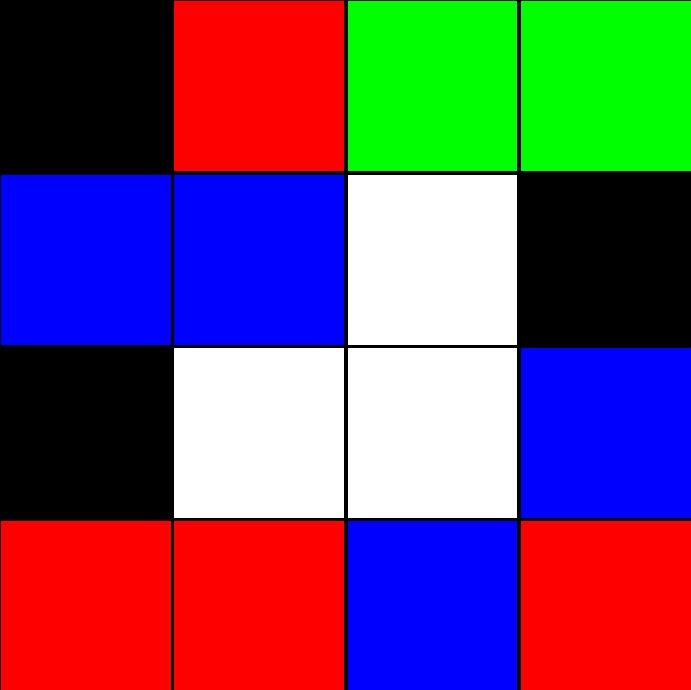
\includegraphics[width=0.3\columnwidth]{Abbildungen/16bit.JPG}
  \end{center}
\end{figure} 

In diesem konkreten Fall wird das Bild zeilenweise von links oben nach rechts unten gescannt und speichert Tupel $T = (L,V)$ mit $L$ hintereinander auftretenden Werten $V \in \{ R,G,B,W,S\}$:

$$RLE = ((1,S),(1,R),(2,G),(2,B),(1,W),(2,S),(2,W),(1,B),(2,R),(1,B),(1,R))$$

Die Werte lassen sich dann wie folgt lesen:
\begin{itemize}
\item $(1,S)$ Ein Pixel Schwarz
\item $(1,R)$ Ein Pixel Rot
\item $(2,G)$ Zwei Pixel Grün
\item $(2,B)$ Zwei Pixel Blau
\item ...\\
\end{itemize}



Verlangt war eine Methode zur Komprimierung mit folgender Signatur:\\
\lstset{language=C, basicstyle=\small,  numbers=left, numberstyle=\tiny}
\begin{lstlisting}[caption={Signatur der compress-Methode},frame=single, captionpos=b, label=code-comm-task, xleftmargin=.03\textwidth]
int compress(char *data, char *result, unsigned int result_size)
\end{lstlisting}
Die Methode erhält einen Pointer auf die unkomprimierten Eingabedaten \textit{data} und speichert die lauflängenkodierten Daten in das char-Array \textit{result}. Der Parameter \textit{result\_size} gibt die maximale Größe des für \textit{result} reservierten Speicherbereichs an.




\subsection{Das Bitmap Format}

\subsubsection*{Genereller Aufbau}

BMP-Dateien bestehen insgesamt aus vier Teilen: dem Dateikopf, dem Informationsblock, der Farbtabelle und den Bilddaten. 

\begin{table*}[h!]
\begin{center}
\caption{Schematischer Aufbau einer Bitmap}
\begin{tabular}{|c|}
\hline
BITMAPFILEHEADER\\
\hline
BITMAPINFOHEADER\\
\hline
RGBQUAD array\\
\hline
Color-index array\\
\hline
\end{tabular}
\end{center}
\end{table*}

\newpage
\subsubsection{Dateikopf}


Der Dateikopf enthält wichtige Randdaten für das File:



\lstset{language=C, basicstyle=\small,  numbers=left, numberstyle=\tiny}
\begin{lstlisting}[caption={Struct: file\_header},frame=single, captionpos=b, label=code-comm-task, xleftmargin=.03\textwidth]
typedef struct {
	char         bfType[2]; 	  // Zeichenkette "BM" (hex: "0x4D42" )											     	Identifiziert die Datei als Bitmap     
	unsigned int bfSize;       // Grösse der Bitmap in bytes (ist konstant 14)	     
	short        bfReserved1;  // Für das System reserviert, immer null   
	short        bfReserved2;  // Für das System reserviert, immer null  
	unsigned int bfOffBits;    // Offset vom Anfang des Dateikopfes zum ersten Eintrag der Bilddaten. * (1)   
} file_header;
\end{lstlisting}

\subsubsection{Informationsblock}

Der Informationsblock spezifiziert Daten, die zum Einlesen der Bitmap benötigt werden:
\lstset{language=C, basicstyle=\small,  numbers=left, numberstyle=\tiny}
\begin{lstlisting}[caption={Struct: info\_header},frame=single, captionpos=b, label=code-comm-task, xleftmargin=.03\textwidth]
typedef struct {
	file_header  fileheader;
	unsigned int biSize;  		 // Grösse der info_header structure in
  										   Bytes (konstant 40)
	int          biWidth;  		// Breite des Bildes in Pixeln
	int          biHeight;		 // Höhe des Bildes in Pixeln * (2)
	short        biPlanes; 		// Immer eins. Nicht verwendet. 
	short        biBitCount;  		// Farbtiefe der Bitmap * (3)
	unsigned int biCompression; 		 // Kompessionstyp * (4)
	unsigned int biSizeImage;  		// Grösse der Bilddaten in Bytes.
	int          biXPelsPerMeter;		 // Horizontale Auflösung des Ausgabegeräts in Pixel pro Meter
	int          biYPelsPerMeter; 		 // Vertikale Auflösung des 																Ausgabegeräts in Pixel pro Meter
	unsigned int biClrUsed;  		// Anzahl der Indizes, die in der Farbtabelle benutzt wurden. 
	unsigned int biClrImportant;		 // Die Anzahl and Farben, die															 benötigt werden um die Bitmap darzustellen
} info_header;
\end{lstlisting}

Anmerkungen: \\

\textbf{* (1) bfOffbits}

Adressiert, dass die Größe der Farbtabelle nicht bei jeder Bitmap gleich ist und der Anfang der Bilddaten als variabler Wert angegeben werden muss.  \\


\textbf{* (2) biHeight} 

Ist biHeight positiv, wird die Bitmap von unten nach oben gelesen; der Ursprung der Bitmap ist die linke untere Ecke. 
Ein negativer Wert in biSize indiziert, dass die Bitmap von oben nach unten zu lesen ist, mit dem Urpsrung in der der rechten oberen Ecke.\\


\textbf{* (3) biBitCount} 

 biBitCount ist ein Wert von 1, 2, 4, 8, 16, 32 oder 64
Der Wert beschreibt die Anzahl der Bits, die zur Kodierung der Farbwerte zur Verfügung stehen. Für Farbtiefe=8 gibt es $2^8$ mögliche Farben\\


\textbf{ * (4) Kompressionstyp}

Der Kompressionstyp kann ein Wert aus [0,3] sein.
\begin{itemize}
\item 0: Bitmap is unkomprimiert
\item 1: Bilddaten sind lauflängenkodiert für 4 Bits per Pixel (bpp). Kompression nur            möglich, wenn biBitcount=4 und biHeight positiv.
\item 2: Bilddaten sind lauflängenkodiert für 8 bpp. Kompression nur möglich, wenn                biBitcount=8 und biHeight positiv.
\item 3: Bilddaten sind unkomprimiert und mittels Farbmasken kodiert.

\end{itemize}

\subsubsection{Farbtabelle}
Es folgt eine Farbtabelle.
Jeder Eintrag in der Farbtabelle ist 4 Byte groß und gibt einen Wert für den Blau-,Grün- und Rotanteil an (die Reihenfolge ist BGR, nicht RGB.). Der vierte Wert wird immer auf 0 gesetzt.\\\\

Die Anzahl der Einträge hängt von biColors ab:
\begin{itemize}
\item Ist biColors gleich null, wird die maximale Anzahl and Farbwerten verwendet, die durch biBitCount zugelassen werden.
\item Ist biColors größer als null, enthält die Farbtabelle so viele Einträge, wie in biColors Used spezifiziert. 
\end{itemize}


\subsubsection{Bilddaten}
\subsubsection*{Bilddaten im unkomprimierten Format}

Für biBitCount = 1, 4, oder 8 werden für jeden Pixel des Bildes der Eintrag in der Farbtabelle angegeben. Die Reihenfolge der Pixel ist durch das Vorzeichen von biHeight gegeben;

\subsubsection*{Bildaten im RLE-8 komprimierten Format}

In einem lauflängencodierten Bild bilden jeweils zwei aufeinanderfolgende Bytes einen Datensatz.\\ Hat das erste Byte einen anderen Wert größer als 0, so wird das zweite Byte, sprich der Pixel mit dem entsprechenden Farbwert, so oft wiederholt, wie das erste Byte angibt. Hierbei befindet man sich im \frqq encoded mode\flqq~. Hat das erste Byte den Wert 0 und das zweite Byte einen Wert $n$, der zwischen 3 und 255 liegt, so werden die nächsten $n$-Bytes als Pixelwerte direkt übernommen und bilden keine Tupel, auch \frqq absolute mode\flqq~genannt. \\

Zusätzlich gibt es in einer lauflängenkodierten Bitmap folgende reservierte Tupel-Kombinationen, um bestimmte Sonderfälle anzuzeigen:

\begin{itemize}
\item $(0,0)$ Dieses Tupel beschreibt das Ende einer Pixelzeile
\item $(0,1)$ Dieses Tupel beschreibt das Ende der Bitmap
\item $(0,2)$ Dieses Tupel beschreibt eine Verschiebung der aktuellen Pixelposition. Die beiden folgenden Bytes geben die Verschiebung nach rechts und nach unten an.
\end{itemize}


\section{Lösungsfindung}

Das Windows Bitmap-Format ist sehr gut dokumentiert. Dementsprechend war unser erster Anlaufspunkt die Windows-Dokumentation und Wikipedia, die beide eine sehr gute Einführung in die Systematik des bmp-Format bieteten. Daraufhin entwickelten wir zuerst ein C-Programm, dass eine Datei im Bitmap Format einlesen konnte und exakt wieder in ein leeres char-Array speicherte, um selber noch einmal nachvollziehen zu können, wie Bitmaps überhaupt aufgebaut sind. Dies bot uns auch das Grundgerüst für die spätere Implementierung des Assembler Codes, da nur die eigentliche Komprimierung darin stattfinden soll.\\
Der nächste Schritt bestand aus Umsetzung der Lauflängenkodierung nur im absoluten Modus in C. Wir wollten dies als Vorlage für den Assembler Code nutzen, nach dem Hinweis das man diesen \glqq per Hand\grqq in Assembler Code übersetzen kann. Auffällig war, dass das Datei des Beispielbildes der Aufgabenstellung in dieser Form größer wurde.\\
Es folgte eine Umsetzung mit beiden Modi, encoded und absolut, in C. Für die Behandlung von Spezialfällen wurde hier der erhöhte Aufwand besonders deutlich, da sowohl für encoded und absolut Mode das Auftreten von gleichen und unterschiedlichen Pixeln anders gehandhabt werden muss. Auch die benötigte Behandlung bei Ende einer Zeile und maximaler Länge eines Laufes ( 255 ) zeigte, dass die Übersetzung in Assembler mit einer hohen Verschachtelung von Vergleichen zurechtkommen muss. Zuanfangs war unklar das auch im absoluten Modus alles in abgeschlossenen Wörtern stehen muss, das heißt ein Lauf mit ungerader Anzahl an Pixeln wird mit einem 0-Byte beendet. Dies wurde auch erst im Vergleich mit dem Bildbeispiel deutlich, nachdem unser Algorithmus kein lesbares Bild lieferte.Dazu betrachten wir folgendes Beispiel:

$$0, 8, 192, 167, 167, 45, 89, 42, 13, 96$$

Bei dieser Folge von Bytes würde uns mit dem Tupel $(0,8)$ angezeigt, dass die folgenden 8 Bytes einzelne Pixel sind und keine Folgen von Farbinformationen beschreiben. Ein Programm, dass die Grafik wieder dekomprimiert, weiß, dass nach 8 Bytes wieder ein Tupel kommt, welches eine Folge beschreibt.

$$0, 7, 192, 167, 167, 45, 89, 42, 13, 0$$

In diesem Beispiel folgt eine ungerade Anzahl an einzelnen Farbinformationen und wird deshalb mit einem 0-Byte aufgefüllt.\\
\\
Nachdem wir eine vollständige Implementierung in C erstellt hatten, wurde zuerst nur der einfache Algorithmus in Assembler übersetzt. Dies diente auch dazu sich mit dem Aufbau und den Methoden vertraut zu machen, die wir brauchen um die vollständige Lauflängenkodierung zu implementieren. Erstmals wurde uns hier klar, dass die vorgebene Definition der Assembler-Methode nicht ausreicht, da in unkomprimierter Form und nur mit der Startposition des Daten-Arrays die Länge des Arrays verloren geht. In unkomprimierter Form gibt es kein Zeichen, das das Ende des Bildes anzeigt, wie die 0 1 -Bytes in komprimierter. Aus diesem Grund haben wir einen weiteren Parameter eingeführt, der die Länge des Daten-Arrays repräsentiert:\\
\lstset{language=C, basicstyle=\small,  numbers=left, numberstyle=\tiny}
\begin{lstlisting}[caption={Neue Signatur der compress-Methode},frame=single, captionpos=b, label=code-comm-task, xleftmargin=.03\textwidth]
int compress(char *data, char *result, unsigned int result_size, unsigned int data_size)
\end{lstlisting}
Der Entscheidende Teil der Lösungsfindung war die Übersetzung des Algorithmus von C in Assembler. Hierzu gingen wir den C-Code Stück für Stück durch. Für jede Condition musste ein Branch in Assembler erstellt werden, der an richtiger Stelle wieder mit dem alternativen Programmlauf zusammenführt. Hierzu wurden die Branches am Ende der Assembler Datei angefügt und in die Gruppen \glqq Encoding-Mode\grqq , \glqq Absolute-Mode\grqq~und \glqq EOF-Mode\grqq~(End Of File) für bessere Lesbarkeit zusammengefasst.\\
Ein Problem das sehr schnell auftrat war die geringe Menge an Standard Registern, die zur Verfügung stand. Grund hierfür sind die vielen Variablen die von uns genutzt werden um State (absolut oder encoding) oder Counter für die runs zu speichern. Eine einfache Lösung sind hier die floating-point Register, s-Register, die wir benutzen um Variablen zu speichern. Dabei nutzen wir diese ausschließlich für Integer und übertragen diese zum lesen und schreiben in ein Standard Register.\\
Die Signatur der compress Methode mussten wir ein weiteres mal ändern, da eine Modulo Operation nicht direkt unterstützt ist. Dies brauchen wir um End-Of-Line festzustellen. Die Breite des Bildes ist indirekt in der Länge des Daten-Arrays enthalten, vorrausgesetzt das Bild ist quadratisch. Dies war beim Beispielbild der Fall, weswegen wir uns entschlossen haben dies als Vorraussetzung für den Algorithmus anzunehmen, um weitere Parameter zu vermeiden. Aus der Breite des Bildes in Parameter 4 können wir die Länge des Daten-Arrays einfacher berechnen als in umgekehrter Reihenfolge, dafür würden wir eine Wurzel berechnen müssen.\\
\lstset{language=C, basicstyle=\small,  numbers=left, numberstyle=\tiny}
\begin{lstlisting}[caption={Endgültige Signatur der compress-Methode},frame=single, captionpos=b, label=code-comm-task, xleftmargin=.03\textwidth]
int compress(char *data, char *result, unsigned int result_size, unsigned int width)
\end{lstlisting}
Durch testen (s. Kapitel \ref{sec:ergebnisse} auf S.\pageref{sec:ergebnisse}) konnten wir die Korrektheit unser Implementierung verifizieren und haben festgestellt, das keine Strukturverändernden Methoden nötig waren, um den Algorithmus von C in Assembler zu übertragen.


\section{Dokumentation der Implementierung}


\subsection{Lesen und Schreiben der Bitmap}

Zum Lesen und Schreiben von Bitmaps verwenden wir das Struct \textit{bitmap}, welches kompakte Handles auf die Datenblöcke der Input-Bitmap bereitstellt.


\begin{lstlisting}[caption={Struct: bitmap},frame=single, captionpos=b, label=code-comm-task, xleftmargin=.03\textwidth]
typedef struct {
	info_header* pInfo;
	file_header pFile;
	unsigned char *data;
	unsigned char* colorTableData;
} bitmap;

\end{lstlisting}



Die Methode  $readBitmap$   bekommt als Parameter den Namen der Input-Datei und ein leeres bitmap-Struct übergeben. Sie öffnet das Input-File und liest daraus File-und Infoheader in das entsprechende Struct ein. Farbtabelle und Bilddaten werden ebenso in das jeweilige Array eingelesen.\\
\begin{lstlisting}[caption={Signatur der Methode readBitmap},frame=single, captionpos=b, label=code-comm-task, xleftmargin=.03\textwidth]
readBitmap(char* name, bitmap* bm)
\end{lstlisting}


Die Methode $writeBitmap$ öffnet ein neues File mit Namen, der als Parameter übergeben wurde. Analog zur read-Methode werden nacheinander File- und Infoheader, Farbtabelle und Pixeldaten in das File geschrieben. Während sich im bitmap-Struct die Bitmap-Header und die Bilddaten durch das Komprimieren geändert haben, wird die Farbtabelle so wie eingelesen übernommen.\\
\begin{lstlisting}[caption={Signatur der Methode writeBitmap},frame=single, captionpos=b, label=code-comm-task, xleftmargin=.03\textwidth]
writeBitmap(char* name, bitmap* bm)
\end{lstlisting}


\subsection{Algorithmus zur Lauflängenkodierung}
Sowohl in Assembler, als auch in C hat der Algorithmus zur Lauflängenkodierung die gleiche Struktur. Dies hat den Ursprung vor allem in der direkten Übertragung von C nach Assembler.\\
Zunächst sind einige Variablen definiert, die dazu dienen Stati zu speichern. Über diese ist definiert, ob sich der momentane Lauf im absoluten oder encoding Modus befindet und wie lang die entsprechenden Läufe, bzw. wie viele Pixel enthalten sind:
\begin{lstlisting}[caption={Variablen},frame=single, captionpos=b, label=code-comm-task, xleftmargin=.03\textwidth]
unsigned char current = bm->data[0]; // Aktueller Pixel
unsigned char last; // Letzter Pixel

int run = 0; // Anzahl von aufeinanderfolgenden gleichen Pixeln
int resultIndex = 0; // Position im result-Array
int isAbsoluteMode = 0; // Aktueller Modus, 0 encoding, 1 absolut
int absoluteStartIndex = 0; // An welchem Index wurde der Indikator für den absoluten Lauf ( 0 ) gespeichert
int absoluteRun = 0; // Anzahl an Pixeln die im absoluten Lauf gespeichert werden
int forceNormal = 0; // Bestimmt, ob auch bei run < 3 im encoding Modus gespeichert werden soll
\end{lstlisting}
Das Daten-Array wird nun durchlaufen und ein neuer Pixel eingelesen. Die Variable run wird um eins erhöht, da dies in jedem Fall nötig ist. Zunächst wird nun unterschieden in welchem Modus man sich befindet. Dies geschieht zuerst, da alle nachfolgenden Handlungen sich je nach Modus unterscheiden. Die Reihenfolge der nachfolgenden Schritte ist für beide Modi gleich, müssen allerdings unterschiedlich gehandhabt werden:
\begin{itemize}
\item Überprüfung auf Ende einer Reihe
\item Vergleich von last und current
\item Überprüfung auf maximale Lauflänge
\end{itemize}
Nachdem alle Pixel gelesen wurden, muss anschließend noch der offene Lauf beendet und die End-Of-File Bytes angefügt werden. Die drei Möglichkeiten bestehen hierbei aus einem Lauf im encoding Modus, d.h. mindestens die beiden letzten Pixel sind gleich oder nur der letzte ist anders, ein absoluter Lauf mit mindestens drei Pixeln (einschließlich dem letzten), oder nur zwei verschiedene, einzelne Pixel. Entsprechend werden die Läufe beendet und gespeichert.

\subsubsection{Überprüfung auf Ende einer Reihe}
Bei der Überprüfung auf Ende einer Reihe kann im encoding Modus einfach gespeichert werden, im absoluten Modus muss hier unterschieden werden, ob der Lauf lang genug zum speichern ist ( neuesten Pixel anfügen und beenden ) oder hier zwei einzelne verschiedene Pixel vorliegen. Es können nur verschiedene Pixel sein, da bei einem einzelnen noch nicht in den absoluten Modus gewechselt wird. Die tatsächliche Überprüfung, ob die Pixel gleich sind findet erst später statt. Der aktuelle Pixel muss auch nicht beachtet werden, da dieser sich schon in der nächsten Reihe befindet. Beispielsweise wenn die Breite 512 Pixel beträgt, ist Pixel 511 der letzte einer Reihe. Der Schleifendurchlauf kann hiernach auch neu gestartet werden.
\subsubsection{Vergleich von last und current}
Für den encoding Modus bedeutet die Überprüfung von aktuellem und letztem Pixel, muss der Lauf beendet werden und wenn ja, ist dieser lang genug. Für eine Länge von unter 2 Pixeln soll ein absoluter Modus verwendet werden, dies bedeutet eine Platzersparnis, es sei denn er ist umschlossen von einer großen Anzahl an gleichen Pixeln, hier repräsentiert durch \glqq forceNormal\grqq .\\
Im absoluten Modus wird bei unterschiedlichen Pixeln dieser einfach an den Lauf angefügt und gespeichert. Für den Fall von gleichen wird erst ab drei aufeinanderfolgenden der Lauf beendet und je nach Gesamtlänge des Laufes in einzelne Tupel gespeichert ( forceNormal ) oder beendet. Hierzu muss die Anzahl der Pixel an der vorgesehenen Stelle ( absoluteStartIndex +1 ) gespeichert und der optionale 0-Byte, bei ungerader Anzahl, angefügt werden.
\subsubsection{Überprüfung auf maximale Lauflänge}
Am Ende jedes Schleifendurchlaufes wird überprüft, ob die Länge des Laufes 255 erreicht hat, da in einem 8-Bit pro Pixel komprimierten Bild nur Zahlen bis 255 gespeichert werden können. Sollte dies der Fall sein, werden die Läufe einfach beendet und die Werte gespeichert. Auch hier wird, wie immer wenn ein Lauf beendet wird, der Modus auf encoding gesetzt. Dies dient dazu das Handling zu vereinfachen, da bei einem aboluten Lauf, der vorzeitig beendet wird Pixel überschrieben werden müssen, aus dem Grund das jeder gelesene Pixel in diesem Modus sofort gespeichert werden muss.

\subsection{Benutzer-Dokumentation}
Zum testen der Implementierung kann man wählen zwischen Implementierung in C und Assembler. Diese befinden sich den den Ordnern:
\begin{itemize}
\item compressInASM
\item compressInC
\end{itemize}
In beiden Ornder befindet sich ein Makefile das sich mit make ausführen lässt. Das komprimierte Lena-Bild befindet sich dann in diesem Ordner. Ursprung und Zieldatei des Bildes steht hardgecoded am Ende der c-Datei in der Main.
Die auszuführenden Programme erwarten einen Paramter. Dieser gibt die Anzahl an, wie oft die Komprimierung durchgeführt wird, um eine durchschnittliche Zeit zu berechnen. Dies würde in den Ordnern so aussehen:
\begin{itemize}
\item compressInASM: ./asmCompress 100
\item compressInC: ./compressInC 100
\end{itemize}
Die respektiven Befehle stehen hinter dem Doppelpunkt. Die Anzahl der Durchläufe kann angepasst werden.

\section{Ergebnisse}\label{sec:ergebnisse}

Um die Laufzeiten vom Assembler-Code, der die Lauflängencodierung implementiert, gegen die C-Implementierung zu testen, wurden beide Programme 100-mal ausgeführt und die durchschnittliche Laufzeit in Sekunden errechnet. Der C-Code benötigt dabei im Mittel für eine Komprimierung eine Zeit von 0,0245 Sekunden. Der Assembler-Code hingegen nur 0,0135 Sekunden. Dies entspricht einer Zeitersparnis von fast 44,9 \%.\\
\\
Die unkomprimierte  Version des Bildes hat eine Größe von 263 kB, während die Größe der komprimierte Datei  248 kB beträgt. Es wurde eine Kompressionrate von 5,7\% erzielt, was 15 Kilobyte entspricht. Hierbei war auch keine größere Kompression zu erwarten, da unser vorgegebenes Testbild kein Paradebeispiel für die Kompressionseffizienz der Lauflängencodierung ist. Dafür hat es zu kleine Flächen mit der gleichen Farbe und ist insgesamt zu detailreich.

\section{Zusammenfassung und Ausblick}

Die Lauflängencodierung (Run-Length-Encoding) ist ein verlustfreier Kompressionsalgorithmus, der redundante Daten in Form von Wiederholungen beseitigt und sich besonders für Bilddateien mit großen Farbflächen mit wenigen Einzelfarben eignet. Gerade bei Schwarz-Weiß-Seiten erziehlt das Kompressionsverfahren gute Ergebnisse, weshalb es unteranderem in der Fax-Übertragung seinen Einsatz findet. Die RLE-Kodierung ist umso ungeeigneter, je detailreicher die Grafik ist. Grundsätzlich zeichnet sich die Codierung aber durch ihre Einfachheit und Geschwindigkeit aus.

\newpage
\section{Quellenverzeichnis}

\subsection{Fachliteratur}

\begin{itemize}
\item Uwe Baumgarten. \textit{Präsentationsfolien zu \frqq Betriebssysteme und hardwarenahe Programmierung für Games\flqq}
\item Übungsfolien des Praktikums \textit{Aspekte der systemnahen Programmierung bei der Spieleentwicklung}

\end{itemize}

\subsection{Internetliteratur}

\begin{itemize}
\item Bitmap Compression:\\https://msdn.microsoft.com/de-de/library/windows/desktop/dd183383(v=vs.85).aspx
\item BITMAPFILEHEADER:\\https://msdn.microsoft.com/de-de/library/windows/desktop/dd183374(v=vs.85).aspx
\item BITMAPINFOHEADER:\\https://msdn.microsoft.com/en-us/library/windows/desktop/dd318229(v=vs.85).aspx
\item RGBQUAD array:\\https://msdn.microsoft.com/de-de/library/windows/desktop/dd162938(v=vs.85).aspx
\end{itemize}

\end{document}